% === Concepts of Accelerator Physics
\chapter{Concepts of Accelerator Physics}
\thumbforchapter{}
\chaptertoc{}
\newpage

\begin{enumerate}
    \tightlist
    \color{red}
    \item Coordinates
    \begin{enumerate}
    \tightlist
        \item Linear Maps
        \item Normal Form \& RDT \& resonance diagram
    \end{enumerate}
    \item Chromaticity
    \begin{enumerate}
    \tightlist
        \item Combined effect of multipoles
        \item Amplitude Detuning
        \item Chromtic Amplitude Detuning
        \item Dynamic Aperture
    \end{enumerate}
    \item Luminosity
\end{enumerate}



\input{chapters/02_Background/introduction.tex}
\section{Magnetic Fields}

% ============================================
%                Nomenclature
% ============================================
\subsection{\review{Nomenclature}}

Several notations coexist to denote magnetic fields. In this thesis, the
\textit{European Convention}~\cite{dilly_corrections_2022} is used for field indices, as shown
in Tab.~\ref{tab:magnetic_fields:relation_indices}. MAD-X, and MAD-NG, however, use the
\textit{American Convention}.

\begin{table}[H]
    \centering
    \begin{tabular}{l|c|c|c}
        Multipole     &      MAD-X        &     Index        & Normalized Strength \\
    \hline            
        Dipole        &     0             &     1            & $K_1$   \\       
        Quadrupole    &     1             &     2            & $K_2 $  \\
        Sextupole     &     2             &     3            & $K_3 $  \\
        Octupole      &     3             &     4            & $K_4 $  \\
        Decapole      &     4             &     5            & $K_5 $  \\
        Dodecapole    &     5             &     6            & $K_6 $  \\
        Decatetrapole &     6             &     7            & $K_7 $  \\
    \end{tabular}
    \caption{Relation between field indices and multipoles.}
    \label{tab:magnetic_fields:relation_indices}
\end{table}

As such, unless explicitly stated, quantities such as the magnetic strength $b$ and normalized
strength $K$ will be expressed with this notation. 


% ============================================
%              Multipole Expansion
% ============================================
\subsection{\review{Multipole Expansion}}

A 2 dimension magnetic field in the planes \textit{x} and \textit{y} can be described as a sum of
the normal and skew field gradients $\mathcal{B}$ and $\mathcal{A}$ with multipoles of order $n$,
given by~\cite{wolf_engineering_2001}:
\begin{equation}
    B_y + iB_x = \sum_{n=1}^\infty \left(\mathcal{B}_n + i\mathcal{A}_n \right)  (x+iy)^{n-1}
\end{equation}

An ideal magnet would produce either a sole normal or skew field. However, this is not applicable 
to real-life magnets that are imperfect, due to design and manufacturing constraints.
Field errors are thus introduced, relative to the main field of the ideal 2N-pole magnet at a
reference radius $r_{ref}$~\cite{dilly_corrections_2022}, as shown in 
Eq.~\eqref{eq:magnetic_field:relative_errors}. The coefficients of the normal and skew relative 
field errors, referred to as $a_n$ and $b_n$, are dimensionless but often given in \textit{units}
of $10^{-4}$.

\begin{equation}
    B_y + iB_x = 
        \begin{cases}
            \mathcal{B}_N \cdot \sum_{n+1}^\infty (b_n + ia_n) \left(\frac{x+iy}{r_{ref}}\right)^{n-1}\text{, for normal magnets}\\
            \mathcal{A}_N \cdot \sum_{n+1}^\infty (b_n + ia_n) \left(\frac{x+iy}{r_{ref}}\right)^{n-1}\text{, for skew magnets}
        \end{cases}
    \label{eq:magnetic_field:relative_errors}
\end{equation}


The normal and skew field components of order $n$ for an imperfect 2N-pole magnet is thus given by
the following equation:

\begin{equation}
    \begin{aligned}
        \mathcal{B}_n &= \mathcal{B}_N \cdot \frac{b_n}{r_{ref}^{n-1}}, \\
        \mathcal{A}_n &= \mathcal{A}_N \cdot \frac{a_n}{r_{ref}^{n-1}}.
    \end{aligned}
\end{equation}

The unit of the field is relative to the multipole order $n$: $[\text{Tm}^{1-n}]$.


% ============================================
%              Normalization
% ============================================
\subsection{\review{Beam Rigidity and Normalization}}

\subsubsection{\review{Beam Rigidity}}

The beam rigidity refers to the resistance of a particle moving through the accelerator to the
bending applied by the magnetic fields. It is derived from the Laurentz force~\cite{dilly_corrections_2022}
and relates the magnetic field $B$, the radius of curvature $\rho$ to the momentum $p$ and charge $q$
of the particle:

\begin{equation}
    B \rho = \frac{p}{q}
    \label{eq:magnetic_fields_beam_rigidity}
\end{equation}

It is of interest when designing an accelerator to set the maximum field as well as the required
radius of curvature for a specific momentum and particle.
An interesting metric of an accelerator is also its \textit{filling factor}, or percentage of
dipoles in the machine. It can be calculated via the radius of curvature: $f = \rho / r$. A low 
filling factors means more space for other magnets, collimators, beam instrumentation, etc.

\subsubsection{\review{Field Normalization}}

The Beam Rigidity is also used as a way to normalize magnetic field strengths in particle
accelerators where the momentum of the particle changes (i.e. acceleration).
Normalized Normal and Skew components $K_n$ and $J_n$ are given by~\cite{wolf_engineering_2001}:

\begin{equation}
    \begin{aligned}
        K_n =  \frac{q}{p} &(n-1)! \mathcal{B}_n, \\ 
        J_n =  \frac{q}{p} &(n-1)! \mathcal{A}_n.
    \end{aligned}
    \label{eq:magnetic_fields_normalized}
\end{equation}



% ============================================
%            Hamiltonian Dynamics
% ============================================
\subsection{Hamiltonian Dynamics}

\todo{link to lie algebra\\
poisson bracket is a link between hamiltonian and coordinate evolutions \\
Lie Algebra uses poisson brackets}

The Hamiltonian describing the motion for the transverse planes of a given multipole or order $n$ is
given by~\cite{keintzel_jacqueline_beam_nodate,tomas_direct_2003,franchi_studies_2006}:

\begin{equation}
    \begin{aligned}
        H &= \frac{q}{p} \Re \left[ \sum_{n>1} (\mathcal{B}_n + i\mathcal{A}_n) \frac{(x+iy)^n}{n} \right] \\
          &= \Re \left[ \sum_{n>1} (K_n + iJ_n) \frac{(x+iy)^n}{n!} \right].
    \end{aligned}
    \label{eq:hamiltonian_magnet}
\end{equation}

Quite often, when studying the effect of a magnet on the beam, only one component is required, and
the sum can thus be dropped.
The normal and skew fields can also be isolated in order to consider their effect only:

\begin{equation}
    \begin{aligned}
        N_n &= \frac{1}{n!} K_n \Re \left[ (x+iy)^n \right] \\
        S_n &= -\frac{1}{n!} J_n \Im \left[ (x+iy)^n \right].
    \end{aligned}
    \label{eq:normal_skew_hamiltonian_magnet}
\end{equation}




\section{Coordinate Systems}

In circular accelerators, particle dynamics are represented using a traveling coordinate system.
A reference orbit is determined by the lattice and its magnet strengths, forming the
\textit{optics}. In the case of a synchrotron, like the LHC, where the particles return to their
original location after some turns, the reference orbit is also called the closed orbit.  
The Frenet-Serret coordinate system is used, moving along the ring on the reference orbit. The
coordinates are then transverse: $x$ and $y$, and longitudinal in the direction of travel: $s$.
Figure~\ref{fig:coordinate_systems:frenet_serret} shows those coordinates.

\begin{figure}[H]
    \centering
    \includegraphics[width=0.6\textwidth]{example-image-a}
    \caption{\todo{Frenet-Serret coordinates commonly used in accelerator physics.}}
    \label{fig:coordinate_systems:frenet_serret}
\end{figure}



% ============================================
%               Linear Lattice 
% ============================================
\subsection{Linear Lattice}

A circular accelerator is composed of many multipoles of different orders. A basic
design only requires dipoles and quadrupoles in order to operate. Dipoles are used to bend the
particles in order to form the ring, whereas quadrupoles are used to focus the beam to a focal
point, similar to light optics.
Those elements can be arranged in a particular order, to form a \text{FODO} cell. Such cells present
an alternating placement of focusing an defocusing quadrupoles with dipoles in between, as shown in
Fig.\ref{fig:coordinate_systems:fodo}, and are usually repeated many times along the ring.

\begin{figure}[H]
    \centering
    \includegraphics[width=0.6\textwidth]{example-image-a}
    \caption{\todo{FODO cell, a repeated basic block present in most circular accelerators.}}
    \label{fig:coordinate_systems:fodo}
\end{figure}

A lattice composed on of only dipoles and quadrupoles, is referred to as a \textit{linear} lattice.

\todo{
    Courant Snyder/Twiss
    Tune, beta function
% 
    Lie, normal form
    Resonance Driving Terms
}
\section{Beam Observables}

\todo{title?\\
Linear observables\\
Optics}

% ============================================
%               Dispersion
% ============================================
\subsection{\review{Dispersion}}

Treating a beam as a single particle having the design momentum $p_0$ leads to a machine with no
apparent ill effect related to that momentum.
However, when considering a particle beam where each particle follows a distribution in
momentum, a few effects arise from this deviation, called the \textit{momentum offset},
$\delta$. It is defined as a relative difference to the design momentum:

\begin{equation}
    \delta = \frac{p - p_0}{p_0}.
    \label{eq:coordinate_systems:momentum_offset}
\end{equation}

Those effects are referred to as \textit{chromatic aberrations}. The first and most important to
consider is the \textit{dispersion}. Dispersion results from a particle with a momentum offset
being deflected differently by the dipoles compared to a particle at the design momentum.
Figure~\ref{fig:coordinate_systems:dispersion} shows an example of deflection. 

\begin{figure}[H]
    \centering
    \includegraphics[width=0.6\textwidth]{images/dipole.pdf}
    \caption{Particles with a momentum offset will be deflected differently by dipoles. This offset
            in position can be described by the dispersion function.}
    \label{fig:coordinate_systems:dispersion}
\end{figure}

The particle is still subject to the other properties of the lattice, but with a different orbit,
described by Eq.~\eqref{fig:coordinate_systems:dispersion}.

\begin{equation}
    \begin{aligned}
    D_x(s) = \frac{\Delta x(s)}{\delta} \\
    D_y(s) = \frac{\Delta y(s)}{\delta} \\
    \end{aligned}
    \label{eq:coordinate_systems:dispersion}
\end{equation}



% ============================================
%               Beta Function
% ============================================
\subsection{\todo{$\beta$-function}}

As seen previously in~\ref{section:courant_snyder}, the $\beta$-function is related to the amplitude
of oscillations of the beam. Figure~\ref{fig:beam_optics:beta} shows how the $\beta$-function
oscillates along the ring due to quadrupoles focusing and defocusing properties.
The $\beta$-function is an important quantity found as a factor in several other observables that
will be described later in this thesis.


\begin{figure}[H]
    \centering
    \includegraphics[width=0.9\textwidth]{images/beta_function.pdf}
    \caption{Evolution of the $\beta$-function along the lattice. Horizontal and vertical beatings
    are usually opposite given the focusing and defocusing properties of quadrupoles in each plane.}
    \label{fig:beam_optics:beta}
\end{figure}

A difference in $\beta$-function compared to the design leads to possible unstable and larger beams,
degrading its properties and making it harder to control. The relative difference in
$\beta$-function is called the beta-beating, expressed in percents: 

\begin{equation}
    \mathrm{beating \; [\%]}  = \frac{\beta_z(s) - \beta_z(s)_{model}}{\beta_z(s)_{model}}.
    \label{eq:beam_optics:beating}
\end{equation}


% ============================================
%                  Coupling
% ============================================
\subsection{\review{Coupling}}

In a perfect scenario, the particle motion of each transverse plane is independent, or
\textit{uncoupled}. In practice, this transverse motion can be altered by some magnetic elements,
giving rise to \textit{betatron coupling} where the motion of each plane is not independent anymore.
Such elements can be quadrupoles, mounted with a roll error introducing skew-quadrupolar fields,
which are the main source of coupling in the LHC~\cite{felix_soubelet_local_2023}. Field
imperfections, solenoids and feed-down from higher orders can also contribute to coupling.

The resonances $Q_x + Q_y$ and $Q_x - Q_y$, called the \textit{sum} and \textit{difference}
resonances, are mainly excited by skew quadrupoles. When coupling is present in the
machine, the former may lead to unstable motion while the latter introduces an periodic exchange of
emittance between the planes, keeping it stable. They can be characterized by the RDTs $f_{1010}$
and $f_{1001}$.

Effects of normal multipoles start showing their skew counterpart (and vice versa) as the motion
of transverse planes become coupled. This is demonstrated in \cref{chapter:skew_octupole_fields}
with skew-octupolar RDTs contributed to by normal octupoles in the presence of coupling.


% ============================================
%         Momentum Compaction Factor
% ============================================
\subsection{\todo{Momentum Compaction Factor}}
\label{subsection:coordinates_systems:momentum_compaction_factor}

In synchrotrons, particles with a deviation in momentum with respect to the reference particle will
experience a different path length due to the bending of the dipoles. This effect is characterized
by the \textit{momentum compaction factor}~\cite{keintzel_jacqueline_beam_nodate},

\begin{equation}
    \alpha_c = \frac{\Delta C / C}{\delta},
\end{equation}

relating the circumference of the ring $C$ to the momentum offset $\delta$.
A positive momentum compaction factor indicates a longer path traveled by particles with a positive
momentum offset, and vice versa.


The momentum compaction factor can also be broken down into orders as an infinite sum, where the
linear term is often referred to as the first order,

\begin{equation}
    \alpha_c = \underbrace{\alpha_{c,0}}_{\text{Linear term}}
               + \underbrace{\sum_{i \geq 1} \alpha_{c, i} \delta^i}_\text{Non linear terms}.
\end{equation}

In the LHC, the contribution from the non linear terms is
negligible~\cite{keintzel_jacqueline_beam_nodate}. Further details can be found
in~\cref{subsection:decapoles:chromaticity:measurement}.
\section{Resonances}


%----------------------------------------
%
%----------------------------------------

\begin{figure}[H]
    \centering
    \includegraphics[width=0.7\textwidth]{images/resonance_diagaram_n5.png}
    \caption{Tune diagram with resonances lines excited by multipoles up to decapole ($n \leq 5$).
             The working point of the machine is chosen in an area where few lines are present.}
    \label{fig:resonances:diagram_n5}
\end{figure}


\begin{figure}[H]
    \centering
    \includegraphics[width=0.7\textwidth]{images/resonance_diagaram_n7.png}
    \caption{Tune diagram with resonances lines excited by multipoles up to decatetrapole 
             ($n \leq 7$). When considering higher orders, it becomes apparent that the beam will
             hit several resonances.}
    \label{fig:resonances:diagram_n7}
\end{figure}
\section{Detuning Effects}


% ============================================
%                Chromaticity
% ============================================
\subsection{\review{Chromaticity}}

Chromaticity is the tune change $\Delta Q$ relative to the momentum offset $\delta$. Chromaticity
can be described by a Taylor expansion, given by

\begin{equation} 
    Q (\delta) = Q_0 + Q' \delta + \frac{1}{2!} Q'' \delta^2 + \frac{1}{3!} Q''' \delta^3 + \mathcal{O}(\delta^4).
    \label{eq:background_chromaticity}
\end{equation}

Or, more generally, rewritten as a sum to include all orders up to $n$:

\begin{equation}
    Q (\delta) = Q_0 + \sum_{i=1}^n \frac{1}{i!} Q^{(i)} \delta^i.
    \label{eq:background_chromaticity_sum}
\end{equation}


The first order of the chromaticity expansion, $Q'$, is generally simply referred to as 
\textit{chromaticity}, sometimes as \textit{linear chromaticity}.
The other terms are thus referred to as \textit{non-linear chromaticity}.

The chromaticity change induced by a single element of order $n$ and length $L$ can be derived from
the Hamiltonian of Eq.~\eqref{eq:hamiltonian_magnet}, averaging over the phase variables and
differentiating relative to the actions $J_{x,y}$ and the momentum offset $\delta$:

\begin{equation}
    \Delta Q^{(n)}_{x,y} = \frac{\partial^n Q_{x,y}}{\partial^n \delta} = 
      \frac{1}{2\pi} \int_L \left< \frac{\partial^{(n+1)} H}{\partial J_{x,y}\partial^n \delta}\right> \diff s.
    \label{eq:background_chroma_order_hamiltonian}
\end{equation}


% =========
\subsubsection{Natural Chromaticity from Quadrupoles}

In a purely linear lattice, the linear chromaticity, $Q'$, is a result of the momentum dependence 
of the quadrupoles' focusing. It is in this case called the \textit{natural chromaticity} and can be
derived from the normal hamiltonian of Eq.\eqref{eq:normal_skew_hamiltonian_magnet} and expressing
the normalized magnet strength $K$ with a dependence on $\delta$ via $P$ as $P_0(1+\delta)$:

\begin{equation}
    K_n = \frac{q}{P_0} \frac{1}{1 + \delta} (n - 1)! B_n
    \label{eq:k_dpp}
\end{equation}

The normal field of a quadrupole is then given by

\begin{equation}
    \mathcal{N}_2(x,y) = \frac{1}{2} \frac{q}{P_0} \frac{1}{1+\delta} B_2 (x^2 - y^2)
\end{equation}

By operating a variable change to the angle coordinates 
(\(x \rightarrow \sqrt{2 J_x \beta_x} \cos \phi_x\) and
\(y \rightarrow \sqrt{2 J_y \beta_y} \cos \phi_y\)), the following equation linking the $\beta$-function
and $\delta$ to the normal field is obtained:
\begin{equation}\mathcal{N}_2 (x,y) = \frac{1}{2} \frac{q}{P_0} \frac{1}{1+\delta} B_2 
        \left[
            \left(\sqrt{2 J_x \beta_x} \cos \phi_x \right)^2 
            - \left(\sqrt{2 J_y \beta_y} \cos \phi_y\right)^2
        \right].
    \label{eq:hamiltonian_quadrupole_angle}
\end{equation}

Following Eq.\eqref{eq:background_chroma_order_hamiltonian}, the natural chromaticity $Q'$ induced by
quadrupoles is given by:
\begin{equation}
    \begin{aligned}
        \Delta Q'_x &= \frac{1}{2\pi} \int_L \frac{\partial^2 \left< \mathcal{N}_2 \right> }{\partial J_x \partial \delta} \diff s
        \quad;\quad
        \Delta Q'_y &= \frac{1}{2\pi} \int_L \frac{\partial^2 \left< \mathcal{N}_2 \right>}{\partial J_y \partial \delta} \diff s
        \\
        & = - \frac{1}{4 \pi} \frac{q}{P_0} B_2 L \beta_x
        & = \frac{1}{4 \pi} \frac{q}{P_0} B_2 L \beta_y
    \end{aligned}
\end{equation}


% =========
\subsubsection{Linear Chromaticity from Sextupoles}

The first order chromaticity $Q'$ is contributed to by sextupoles in the presence of off-momentum
particles. The normal field of a sextupole, following Eq.\eqref{eq:normal_skew_hamiltonian_magnet}
is given by

\begin{equation}
    \mathcal{N}_3(x,y) = \frac{1}{3!} (x^3 - 3xy^2).
    \label{eq:detuning:linear_chromaticity}
\end{equation}

As the momentum offset $\delta$ introduces a change in orbit via
dispersion~\cite{keintzel_second-order_2019}, a variable change can be operated on both $x$ and $y$,
as shown in Eq.\eqref{eq:detuning:offset}. In this thesis, vertical dispersion will be though
neglected.

\begin{equation}
    \begin{aligned}
        x &\rightarrow x + \Delta x = x + D_x\delta \\
        y &\rightarrow y + \Delta y = y + D_y\delta
    \end{aligned}
    \label{eq:detuning:offset}
\end{equation}

The positions $x$ and $y$ can once be replaced, using the twiss parameters, giving the full
expression:

\begin{equation}\begin{aligned}
  \mathcal{N}_3(x + \Delta x, y) = \frac{1}{6} K_3 \biggl[&
       \left(\sqrt{2 J_x \beta_x} \cos \phi_x\right)^3 \\
  &    + 3 \left(\sqrt{2 J_x \beta_x} \cos \phi_x\right)^2 D_x \delta \\
  &    + 3 \left(\sqrt{2 J_x \beta_x} \cos \phi_x\right) D_x^2 \delta^2 \\
  &    + D_x^3 \delta^3 \\
  &    - 3 \left(\sqrt{2 J_x \beta_x} \cos \phi_x \right) \left(\sqrt{2 J_y \beta_y} \cos \phi_y \right)^2 \\
  &    - 3 D_x \delta (\sqrt{2 J_y \beta_y} \cos \phi_y)^2 \biggl]
\end{aligned}\end{equation}

Averaging over the phase variables removes any odd cosine:
\begin{equation}\begin{aligned}
  \left< \mathcal{N}_3(x + \Delta x, y) \right> = \frac{1}{6} K_3 &\biggl(
       3 J_x \beta_x D_x \delta \\
  &    + D_x^3 \delta^3 \\
  &    - 3 D_x \delta J_y \beta_y \biggl)
\end{aligned}\end{equation}



The chromaticity can then obtained by differentiating relative to the action $J_{x,y}$ to obtain the
tune, and then by the momentum offset $\delta$.
\begin{equation}
    \begin{aligned}
        \Delta Q'_x &= \frac{1}{2\pi} \int_L \frac{\partial^2 \left< \mathcal{N}_3 \right>}{\partial J_x \partial \delta} \diff s \quad; \quad \Delta Q'_y &&= \frac{1}{2\pi} \int_L \frac{\partial^2 \left< \mathcal{N}_3 \right>}{\partial J_y \partial \delta} \diff s \\
        &= \frac{1}{2 \pi} L \frac{1}{2} K_3 \beta_x D_x  &&= - \frac{1}{2 \pi} L \frac{1}{2} K_3 \beta_y D_x \\
        &= \frac{1}{4 \pi}  K_3 L \beta_x D_x &&= - \frac{1}{4 \pi}  K_3 L \beta_y D_x
    \end{aligned}
\end{equation}

From this last equation, it is apparent than sextupoles are not a source of chromaticity of higher
orders in the presence of linear dispersion. In the presence of second order
dispersion~\cite{keintzel_second-order_2019}, sextupoles can generate some amount of $Q''$, usually
negligible.


% =========
\subsubsection{Non-Linear Chromaticity}

Higher orders of the chromaticity function are described in~\cite{dilly_derivation_2023} and follow
the same logic as for the linear chromaticity from sextupoles.





% ============================================
%             Amplitude Detuning
% ============================================
\subsection{Amplitude Detuning}



% ============================================
%        Chromatic Amplitude Detuning
% ============================================
\subsection{Chromatic Amplitude Detuning}

\todo{make it clear I derived it}